\chapter{Low-Connectivity Reservoirs}\label{ch:low-connectivity}

The choice of ESN meta-parameters that best fits a given task is
difficult to identify. In the absence of strong guiding rules, a
practical approach is to treat it as an optimization problem. In this
chapter, I explore using ESNs on the chaotic system forecasting task
for the Lorenz '63 system, the R{\"{o}}ssler system, and the
double-scroll circuit system described in \cref{ch:systems}. This
exploration is guided by optimization -- by trying to discover the
meta-parameters that result in the best averaged NRMSE
$\tilde{\epsilon}$ during forecasting for the given system. This
exploration leads to a surprising discovery: that ESNs with simple
internal structure perform as well as their more complicated
siblings. In the process, I find concrete evidence that my new
averaged $\tilde{\epsilon}$ metric is a more reliable indicator of
forecasting quality than $\epsilon_1$.

In particular, I am interested in the recurrent connectivity $k$. In
software simulations, such as those described in this dissertation, the
connectivity $k$ has only a slight impact on the speed of the
simulation. However, in hardware network implementations, each
connection has an associated cost. For autonomous Boolean networks
implemented on FPGAs, every network connection is built from a long
chain of delay nodes~\cite{canaday2018}. These delays often compose the
majority of the resource budget of the hardware network. Although the
results in this chapter are all software simulation, the particular
focus on the $k$ parameter is done with an eye towards hardware
implementations.

Many techniques have been used previously for ESN meta-parameter
optimization, such as grid search~\cite{rodan2011} and gradient
descent~\cite{jaeger2007}. However, both of these approaches have
drawbacks. Grid search quickly becomes intractable when the number of
dimensions grows, and even after fixing the two functional
meta-parameters $f$ and $\bm{g}$, there are 5 dimensions.
Compounding this problem, the ESN construction is a random
process, and so the resulting measured $\tilde{\epsilon}$ for a given
set of meta-parameters is a random variable. To obtain a meaningful
result, each set of meta-parameters needs to be tested multiple
times. For even a coarse grid search, with 10 trials and 10 points per
meta-parameter, this already means one million trial RCs. Gradient
descent suffers from the randomness of ESN construction as well, for
the same reasons. It is also unsuitable for use with discrete
parameters such as $k$.

One way to mitigate these problems with random ESN construction
is to modify the ESN construction method outlined in
\cref{sec:esn-construction} to front-load the random choices. For
example, once the recurrent weight matrix $W_r$ has been constructed,
the parameter $\rho_r$ can be changed without any random process at
all. By cleverly factoring out the random parts of ESN construction,
it becomes possible to use methods like grid search and gradient
descent without the extra step of multiple random trials. Ultimately,
however, this is optimizing only a single random instantiation of an
ESN, and provides little insight into how the fully random ESN will
perform.

In this chapter, I use Bayesian
optimization~\cite{yperman2016,maat2018}, as implemented by the
\texttt{skopt} Python package~\cite{skopt2018}, to explore which
meta-parameters result in the lowest forecasting error
$\tilde{\epsilon}$ for the three example systems. Bayesian
optimization deals well with both noise and integer parameters like
$k$, is more efficient than grid search~\cite{maat2018}, and works well
with minimal tuning.

\section{Bayesian Optimization}

% FIXME cartoon figure for this?
Bayesian optimization is a technique that finds the
minimum of an objective function $h(\bm{x})$, in this case the
measured error $\tilde{\epsilon}$ of an ESN with meta-parameters
$\bm{x}$, by repeated evaluation. The process starts with a prior
distribution of functions, representing the algorithm's knowledge of
the function $h$. As each new point $\bm{x}$ is evaluated, the
algorithm incorporates this new knowledge and updates its prior
distribution. At the start of the optimization, points are chosen
randomly. This is the exploration phase, where the Bayesian optimizer
gathers data to improve its prior distribution. After
exploration, the optimizer then evaluates points $\bm{x}$ with the
most expected improvement over the best known minimum so far.

This algorithm has a number of drawbacks. Primarily, it is
complicated. The above summary only scratches the surface, and already
suggests a number of parameters to the optimization algorithm that can
be tuned, such as the initial prior distribution of functions. This
complication makes it difficult to directly claim that any minimum
found is the true minimum, and so I emphasize that this algorithm is
used here for exploration. I am interested in ESNs that perform well,
and what they have in common, but not in claiming any ESN as the best
performer possible. For this purpose, the unopinionated defaults of
the \texttt{skopt} package suffice.

The complexity of this optimization algorithm also manifests in run
time. After the exploration phase, calculating the next set of trial
parameters $\bm{x}$ involves minimizing an internal function
calculated from the current prior distribution. This can be quite
computationally expensive, and so Bayesian optimization is only
suitable for use when the objective function $h(\bm{x})$ is expensive
enough to justify the extra work to reduce how often it is
evaluated. This makes it a good fit here for minimizing prediction error
$\tilde{\epsilon}$ as this involves building, training, and testing
an RC each time.

\begin{table}
  \caption{Range of meta-parameters searched using Bayesian optimization.}
  \begin{tabular}{llrcl}
    & Parameter & min & & max \\
    \hline
    $\gamma$ & Leak Rate & 7 & -- & 11 \\
    $\sigma$ & Input Connectivity & 0.1 & -- & 1.0 \\
    $\rho_\text{in}$ & Input Scale & 0.3 & -- & 1.5 \\
    $k$ & Recurrent Connectivity & 1 & -- & 5 \\
    $\rho_r$ & Recurrent Scale & 0.3 & -- & 1.5 \\
  \end{tabular}%
  \label{tab:bayes-ranges}
\end{table}

In this chapter, the Bayesian algorithm repeatedly generates a set of
meta-parameters to test within the ranges listen in
\cref{tab:bayes-ranges}. Larger ranges require a longer
optimization time. I selected these ranges to include values that
existing ESN design heuristics would choose, while also allowing
exploration outside those ranges without a prohibitively long runtime.

During the optimization process, I discover that the optimizer
often finds ESNs with an input connectivity of $k = 1$ that perform as well as ESNs with a
higher $k$. Such networks have an interesting and simple network
structure, and also suggest other simple structures for comparison.

\section{Structure of Low-Connectivity Reservoirs}

First, networks generated with $k = 1$ often have multiple
disconnected components. For higher $k$, this is still possible but
relatively rare, as $k$ controls the number of opportunities for
components in the network to connect. Disconnected components in the
network essentially act as smaller ESNs operating in parallel. This is an
interesting line of research~\cite{pathak2018}, but not one I
investigate further here. In the interest of a more equitable
comparison between $k = 1$ networks and $k > 1$, I discard and
regenerate any networks with more than a single connected component.

\begin{figure}
  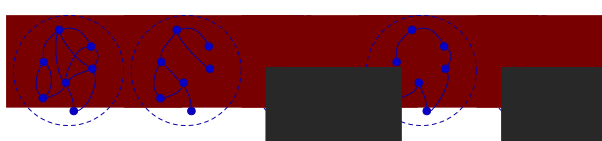
\includegraphics[width=0.7\textwidth]{figures/topology}
  \caption{The five reservoir structures tested. Only internal
    reservoir connections are pictured. Connections to the reservoir
    computer input, or to the output layer are not shown. (a) A
    general, fixed in-degree network, here pictured with $N=7$ and
    $k=2$. (b) A $k=1$ network with a single connected component. (c)
    A $k=1$ network with the single cycle cut at an arbitrary
    point. (d) A \emph{simple cycle reservoir}. (e) A \emph{delay line
      reservoir}.}%
  \label{fig:topology}
\end{figure}

A $k = 1$ network with only a single connected component must also
contain only a single directed cycle. Starting from any node in the
network and working backwards through the single input connection each
node must have will always lead to a single directed cycle, and it is
not possible for two such cycles to exist in the network unless they
are disconnected from each other. This severely limits how recurrence
can occur inside a $k = 1$ network compared to higher-$k$
networks. Every node in a $k = 1$ network is either part of this core
cycle, or part of a directed tree branching off from this cycle, as
depicted in \cref{fig:topology}~(b).

Inspired by the high performance of this simple structure, I also
investigate $k = 1$ networks when the single cycle is cut at a random
point. This turns the entire network into a tree, as in
\cref{fig:topology}~(c). These networks retain the random weights they
have before the single cycle is cut.

Finally, I also investigate reservoir networks that consist entirely
of a cycle or a ring with identical weights with no attached tree
structure, depicted in \cref{fig:topology}~(d), and networks with a
single line of nodes (a cycle that has been cut), in
\cref{fig:topology}~(e). These choices are inspired by the $k = 1$
networks, but have also been researched previously and are known as
\emph{simple cycle reservoirs} and \emph{delay line reservoirs},
respectively~\cite{rodan2011}.

In total, there are five network structures I investigate:
\begin{enumerate}[label= (\alph*)]
\item general construction with unrestrained $k$,
\item $k = 1$ with a single cycle,
\item $k = 1$ with a cut cycle,
\item single cycle, or \emph{simple cycle reservoir},
\item single line, or \emph{delay line reservoir}.
\end{enumerate}
Both the $k = 1$ cut cycle networks (c) and line networks (e) are
rescaled to have a fixed $\rho_r$ before the cycle is cut. However,
after the cycle is cut, they both have $\rho_r=0$. As I
demonstrate in this chapter, these simpler network structures have the capability to
perform as well as their more complicated counterparts, despite the
fact that (c) and (e) have no recurrence and a spectral radius nowhere
near $\rho_r = 1$.

\section{ESN Symmetries and their Consequences}

An ESN in autonomous forecast mode, described by \cref{tab:esn}~(b),
has an inversion symmetry about the origin. That is, if $\bm{r}(t)$ is
a solution to this equation, so is $-\bm{r}(t)$. For an output layer
with an identity read-out function $\bm{g}$, this means that if
$\bm{y}(t)$ is a possible output of the trained RC, then so is
$-\bm{y}(t)$. If the underlying system the ESN is trained to forecast
also exhibits this symmetry, this is not a problem. In fact, designing
the internal reservoir to match symmetries with the input system can
dramatically improve ESN performance~\cite{barbosa2021}.

However, if the input system does not have this symmetry, this can be
an issue. If at any time the autonomous forecast strays near $\bm{r} =
0$, the solution can hop over the symmetry to the other side, and
begin producing an output $\bm{y}(t)$ that is flipped through the
origin. This problem is exacerbated if the input signal $\bm{u}(t)$ is
normalized to have mean zero, a common practice.

This problem is well-known, and a common fix~\cite{pathak2017,herteux2020}
is to use a nonlinear read-out function
\begin{equation}
  g_i(\bm{r}) = \begin{cases}
    r_i & \text{if } i \leq N / 2, \\
    r_i^2 & \text{if } i > N / 2.
  \end{cases}
  \label{eq:esn-break-sym}
\end{equation}
This squares half of the node values before being passed
to the output layer, and breaks the inversion symmetry in the ESN
equation while keeping the number of features accessible to the output
layer the same.

%score: 0.08873905001779689
%score-1: 0.007877037205449461
\begin{figure}
  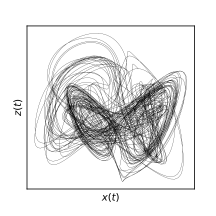
\includegraphics[width=0.6\textwidth]{figures/lorenz-symmetry}
  \caption{The forecasted attractor from an ESN with full inversion
    symmetry trained on the Lorenz '63 system, using identity
    read-out, in the $x$/$z$ plane. Compare against \cref{fig:lorenz},
    and note the two deformed images of the butterfly attractor on top
    of each other, with one flipped along the $z$ axis. Breaking this
    inversion symmetry in the read-out function is enough to prevent
    this kind of failure entirely.}
  \label{fig:lorenz-symmetry}
\end{figure}

This problem can be difficult to diagnose if the input system has a
partial inversion symmetry. For example, the Lorenz '63 system in
\cref{eq:lorenz} has an $(x, y) \rightarrow (-x, -y)$ symmetry, and so
the complete inversion of the Lorenz attractor looks exactly the same
as a flip along the $z$ axis. This is misleading, as the problem has
nothing to do with the Lorenz $z$ variable specifically, and this
confusion prevented a full understanding of the problem until
recently~\cite{herteux2020}. \Cref{fig:lorenz-symmetry} provides an
example of the forecasting failure characteristic to the identity
read-out function when applied to the Lorenz '63 system. The ESN does
a poor job reconstructing the Lorenz attractor, but it also reproduces
this attractor reflected through the origin. This mirror attractor is
not a feature of Lorenz '63, is not present in the training data used
to produce \cref{fig:lorenz-symmetry}, and is entirely due to the
symmetry of the ESN equations. Using the read-out function in
\cref{eq:esn-break-sym} removes this symmetry.

For consistency, I use this \emph{quadratic read-out} for all three
example input systems used in this chapter, even if the inversion
symmetry does exist in the input system as it does for the double-scroll
circuit.

\section{Training, Forecasting, and Evaluation}

Now that I have identified the five networks structures of interest, I
use the Bayesian optimization algorithm to identify networks in each
class that perform well on the system forecasting task. I optimize the
meta-parameters independently for each of the three example input
systems: Lorenz '63, R{\"{o}}ssler, and the double-scroll circuit. I
describe all three systems in \cref{ch:systems}.

For each input system and for each network structure, the Bayesian
algorithm performs random exploration for $50$ iterations, and then
optimization for $50$ iterations, resulting in $100$ iterations in
total. At each iteration of the algorithm, the optimizer constructs a
single random instantiation of an ESN with $N=100$ nodes and the chosen meta-parameters,
trains it, and measures its forecasting performance with the metric
$\tilde{\epsilon}$ defined in \cref{eq:nrmse-avg}. Since the
exploration phase of the optimization is random, I repeat this entire
process 20 times to estimate the variance in the performance of
reservoirs optimized by this method.

To ensure that results are comparable across all three systems, I
normalize their components to have $0$ mean and unit variance. In
addition, I rescale the time axes of all systems so that their maximum
positive Lyapunov exponent matches that of the Lorenz system,
$\lambda_\text{max} = 0.9056$~\cite{viswanath1998}.

To train the ESN, I integrate \cref{eq:esn} with the quadratic readout
in \cref{eq:esn-break-sym}, coupled with the chosen input system, via
the hybrid Runge-Kutta~5(4)~\cite{dormand1980} method from $t = 0$ to
$300$. This produces an ESN response $\bm{r}(t)$. I then divide this interval into three ranges:
\begin{itemize}
\item $t = 0$ -- $100$: the warm-up period,
\item $t = 100$ -- $200$: the training period,
\item $t = 200$ -- $300$: the testing period.
\end{itemize}
As discussed in \cref{sec:training}, the warm-up period is used to
ensure the later times do not depend on the specific initial
conditions of the ESN. I divide the rest into a training period, used
only during training, and a testing period, used later only to
evaluate the ESN performance.

I then determine $W_\text{out}$ via ridge regression, as in
\cref{eq:ridge}, where the sum ranges over the training period. The
ridge parameter $\alpha$ could be included among the meta-parameters
to optimize. However, unlike the other meta-parameters, modifying
$\alpha$ does not require re-integration and can be optimized with
simpler methods.  I select an $\alpha$ from among $10^{-5}$ to $10^5$
by leave-one-out cross-validation, which has an extremely efficient
implementation for ridge regression~\cite{rifkin2007}.
Using the computationally cheaper cross-validation for $\alpha$ instead of the Bayesian algorithm helps to keep the optimizer's computational effort focused on those parameters that most benefit from it.

To evaluate the performance of the trained ESN, I use it to perform
autonomous forecasting using the autonomous equation \cref{tab:esn}~(b). I choose $50$ times
$t_i$ spaced evenly within the testing period. For each $t_i$, I
initialize the reservoir state to $\mathbf{r}(t_i)$, and then
integrate forward with the autonomous equation for one Lyapunov
period, between $t = t_i$ and $t = t_i + 1 / \lambda_\text{max}$. This
produces a reservoir forecast during these times, from which I
calculate an error $\epsilon_{1,i}$ as described in
\cref{eq:nrmse}. Finally, I combine these $50$ errors into a single
$\tilde{\epsilon}$, as in \cref{eq:nrmse-avg}, that represents the
average ability of the ESN to forecast accurately at any point on the
input system attractor.

\begin{figure}
  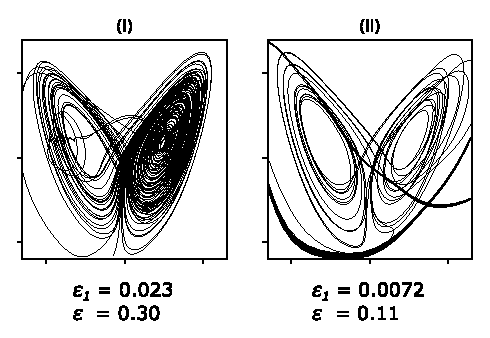
\includegraphics[width=0.6\textwidth]{figures/epsilon-failure}
  \caption{Two examples of ESNs that fail to reproduce
    the Lorenz attractor, but produce a low $\epsilon_1$. Compare with
    the true attractor in \cref{fig:lorenz}. Network (i) fails to
    learn the attractor, overemphasizing the right lobe in which $t_1$
    resides. Network (ii) matches the attractor well early on, but
    as the prediction lengthens, it falls into a periodic orbit (thick
    black line). Both (i) and (ii) show a promising low $\epsilon_1$,
    but the averaged $\tilde{\epsilon}$ measure more accurately
    captures their failure to learn the Lorenz attractor.}%
  \label{fig:epsilon-failure}
\end{figure}

Using $\tilde{\epsilon}$ and not simply $\epsilon_1$ is even more
important in an optimization setting than usual, as searching for ESNs
with the lowest $\epsilon_1$ risks producing ESNs that are only good
at forecasts near $t_1$, but otherwise perform poorly in reproducing
the attractor of their input system. It can also waste time, as the
optimization algorithm explores areas of the parameter space it
believes perform well, but in fact only perform coincidentally well at
$t_1$. \Cref{fig:epsilon-failure} depicts two common ways for an ESN
to fail to replicate the true Lorenz attractor. In
\cref{fig:epsilon-failure} (i), the ESN learns the right lobe of the
attractor reasonably well, as this is where $t_1$ resides, but quickly
exhibits non-Lorenz behavior in the left lobe. In
\cref{fig:epsilon-failure} (ii), the ESN performs well in both lobes
for a short period of time before settling in to a periodic orbit that
does not match Lorenz at all. However, both produce a good short-term
forecast near $t_1$. In particular, network (ii) in
\cref{fig:epsilon-failure} has a lower $\epsilon_1$ than any of the
optimized reservoirs I found despite its obvious failure to learn the
long-term Lorenz attractor.

\section{Results}

\subsection{Forecasting Lorenz '63}

First, I run reservoir networks of all five structures through 100 iterations of
the Bayesian algorithm using the Lorenz system as input, and record
the best-performance RC for each structure according to the metric
$\tilde{\epsilon}$. These reservoirs, and the meta-parameters that
generated them, are reported in \cref{tab:lowk-lorenz-results}. I
estimate the error on $\tilde{\epsilon}$ with the standard deviation of
$\tilde{\epsilon}$ after repeating the optimization process 20 times.

\begin{table}
  \caption{Best reservoir computers of each reservoir structure, after 100
    iterations of the Bayesian optimization algorithm using the Lorenz
    system as input.  The meta-parameters chosen by the algorithm are
    shown on the right. The simpler structures (b) -- (e) all perform
    nearly as well as the general structure (a).}
  \begin{tabularx}{\linewidth}{l l@{\extracolsep{\fill}} l d d d d}
    & & \multicolumn{5}{l}{Lorenz} \\
    & Structure & $\tilde{\epsilon}$ & \multicolumn{1}{c}{$\gamma$} & \multicolumn{1}{c}{$\sigma$} & \multicolumn{1}{c}{$\rho_\text{in}$} & \multicolumn{1}{c}{$\rho_r$} \\
    \hline
    (a) & Any $k$ \footnote{After optimization, $k = 3$.} & 0.022 $\pm$ 0.004 & 7.7 & 0.81 & 0.37 & 0.41 \\
    (b) & $k = 1$ with cycle & 0.024 $\pm$ 0.005 & 10.9 & 0.44 & 0.30 & 0.30 \\
    (c) & $k = 1$ no cycle & 0.028 $\pm$ 0.005 & 7.2 & 0.78 & 0.30 & 0.30 \footnote{\label{fn:lowk-rhor}$\rho_r$ measured before cycle is cut. Afterwards, $\rho_r = 0.$} \\
    (d) & cycle & 0.023 $\pm$ 0.008 & 7.9 & 0.17 & 0.58 & 0.30 \\
    (e) & line & 0.024 $\pm$ 0.003 & 10.6 & 0.79 & 0.30 & 0.45 \footref{fn:lowk-rhor} \\
  \end{tabularx}
  \label{tab:lowk-lorenz-results}
\end{table}

When optimized, all reservoir structures perform well. In particular,
the simpler structures all perform almost as well as the general-$k$
structure. They often lie within one, or at most two standard
deviations from structure (a). This is despite the fact that
structures (c) and (e) both have $\rho_r=0$ and no recurrent
connections within the network. The other structures have
$\rho_r\ll1$.  Previous work has already demonstrated that ESNs with
low or zero spectral radius can still
function~\cite{pathak2017,rodan2011}. These results act as additional
counterexamples to the heuristic that ESNs should have recurrence and
$\rho_r \approx 1$~\cite{lukosevicius2012}.

\subsection{ESN Variation}

These best-observed ESNs are not representative of a
typical ESN.\@ I use the meta-parameters to guide the random input
connections and connections within the network, and so even once the
meta-parameters are fixed, constructing the network is a random
process. Not all networks with a fixed structure type and meta-parameters
will perform the same.

To explore this variation, I generate and evaluate $200$ networks of
each structure on the Lorenz system using the optimized
meta-parameters in \cref{tab:lowk-lorenz-results}. For all five
structures, as the measured $\tilde{\epsilon}$ increases, the quality
of the reproduced attractor decreases gradually. On manual inspection
of the attractors, the reason for this decrease can be divided into
three qualitative regions. For $\tilde{\epsilon} < 0.3$, the RCs
reproduce the Lorenz attractor consistently. Failures still rarely
occur, but they always reproduce part of the attractor before falling
into a fixed point or periodic orbit. In this region, small
differences between the true attractor and the reproduced attractor
contribute more to $\tilde{\epsilon}$ than outright failure. For $0.3
< \tilde{\epsilon} < 1.0$, RCs always fail to reproduce the attractor,
though they will still always reproduce a portion of it before
failing. Examples of these failures are provided in
\cref{fig:epsilon-failure}. Above $\tilde{\epsilon} > 1.0$, these
failures become catastrophic, and no longer resemble the Lorenz
attractor at all. A more quantitative description of these regions is
one line of possible future research.

Though the optimized best-performing networks of
each structure show very little performance difference, the differences
between them become more apparent when we compare the probability
distribution of $\tilde{\epsilon}$ for each topology. These
distributions are shown in \cref{fig:epsilon-distribution}.

\begin{figure}
  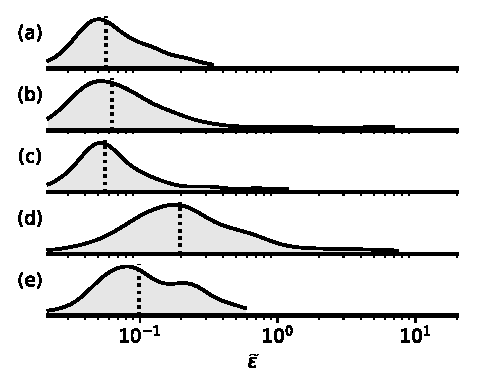
\includegraphics[width=0.6\textwidth]{figures/epsilon-distribution}
  \caption{Performance for each network structure, evaluated for the
    Lorenz system at the meta-parameters listed in
    \cref{tab:lowk-lorenz-results}. Each is visualized as a Gaussian
    kernel density estimation in $\log_{10} \tilde{\epsilon}$ with a bandwidth
    of 0.35~\cite{scott1992}, which can be interpreted as a probability
    distribution. Using a narrower bandwidth does not reveal
    additional features. A vertical line marks the median.  Note that
    structures (b) -- (e) have very long tails, and can produce
    networks that perform very poorly in comparison to (a). However,
    all five have the capability to produce well-performing
    networks.}%
  \label{fig:epsilon-distribution}
\end{figure}

A well-performing network with arbitrary $k$ (a) is a much more
likely outcome than a well-performing network with a single cycle
(d). However, the performance of arbitrary $k$ networks (a) is very
similar to that of tree-like networks (c). Though (c) has a longer
tail on the high end, the simpler structure of the reservoir may be
appealing for hardware RCs.

The distribution of performance for each structure can be a deciding
factor if network construction and evaluation is expensive, as it
might be in hardware. In software, though, I find the
best-performing networks in \cref{tab:lowk-lorenz-results} after only $100$
trials. A hardware design can still benefit from the simpler
structures (b) -- (e) despite their very wide performance distributions
if the creation of the evaluation of the design can be automated to
test many candidate reservoirs, as on an FPGA~\cite{canaday2018}.

There may also be a benefit in software. The simpler structures are
represented by weight matrices $W_r$ in very simple forms. Structure
(c) can always be represented as a strictly lower-diagonal (or upper-diagonal) matrix, and
(d) -- (e) can be represented with non-zero entries only directly below
the main diagonal. Software simulations can take advantage of this structure to
speed up integration of \cref{eq:esn}.

\subsection{Reproducing the Lorenz '63 Attractor}

\begin{figure*}
  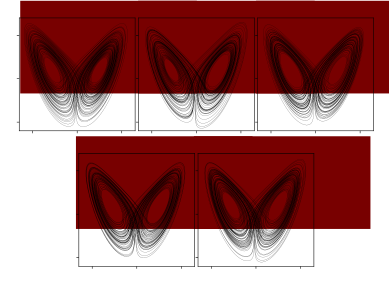
\includegraphics[width=0.7\textwidth]{figures/lowk-attractors}
  \caption{Lorenz attractor plots in the $x$/$z$ plane for long-term
    free-running predictions for each network structure in
    \cref{tab:lowk-lorenz-results}. Compare with true Lorenz attractor
    in \cref{fig:lorenz}, and the failed reservoirs in
    \cref{fig:epsilon-failure}.}%
  \label{fig:lowk-attractors}
\end{figure*}

For each structure I produced a free-running prediction of
the Lorenz system for $100$ time units using the best-performing RC.\@
I use these predictions to produce an attractor as shown in
\cref{fig:lowk-attractors}. All five optimized ESNs reproduce the
Lorenz attractor well. Though comparing these plots by eye is not
quantitative, I find them qualitatively useful: an RC that fails to
reproduce the Lorenz attractor by eye is unlikely to have a low
$\tilde{\epsilon}$ compared to one that does, but visual inspection of
the reproduced attractor can catch rare catastrophic failures that are
not reflected in $\tilde{\epsilon}$.

\subsection{Forecasting R{\"{o}}ssler and the Double-Scroll Circuit}

To explore whether these structures remain equally effective at tasks
beyond forecasting the Lorenz system, I run all five network
structures through 100 iterations of the Bayesian algorithm for both
the R{\"{o}}ssler and the double-scroll systems. As with the Lorenz
system, I estimate the errors on these results by repeating the
process 20 times each. These results are reported in
\cref{tab:lowk-resultsplus}.

\begin{table}
  \caption{Result of optimizing reservoirs with the
      Bayesian algorithm over 100 iterations, on both the
      R{\"{o}}ssler system and the double-scroll system. All five
      structures can perform equally well at both systems.}
  \begin{tabularx}{\linewidth}{l l@{\extracolsep{\fill}} l l}
    & & \multicolumn{1}{l}{Double Scroll} & \multicolumn{1}{l}{R{\"{o}}ssler} \\
    & Structure & $\tilde{\epsilon}$ & $\tilde{\epsilon}$ \\
    \hline
    (a) & Any $k$ & 0.029 $\pm$ 0.006 & 0.017 $\pm$ 0.005 \\
    (b) & $k = 1$ with cycle & 0.033 $\pm$ 0.007 & 0.020 $\pm$ 0.007 \\
    (c) & $k = 1$ no cycle & 0.033 $\pm$ 0.008 & 0.018 $\pm$ 0.006 \\
    (d) & cycle & 0.033 $\pm$ 0.007 & 0.018 $\pm$ 0.006 \\
    (e) & line & 0.037 $\pm$ 0.01 & 0.019 $\pm$ 0.015
  \end{tabularx}
  \label{tab:lowk-resultsplus}
\end{table}

The results for the double-scroll and R{\"{o}}ssler systems agree well
with those for Lorenz. All five structures optimize reliably with the
Bayesian algorithm, and all perform similarly when
optimized. Optimizing a network to reproduce either system will almost
always work after only 100 iterations, regardless of networks
structure.

\subsection{Cross-task Performance}

As RC training is computationally cheap, one advantage to RCs is that a single reservoir can be quickly re-used on many
different tasks by re-training $W_{\text{out}}$. To evaluate whether
this is possible with these optimized networks, I take each of the 20 networks
optimized for the Lorenz system and re-train $W_{\text{out}}$
to instead reproduce the double-scroll circuit system. Every other
part of the RC is left unchanged. I then evaluate how accurate this
prediction is using the metric $\tilde{\epsilon}$. These results are
summarized in \cref{tab:lowk-resultsgen}.

\begin{table}
  \caption{Result of re-using reservoirs optimized for
      Lorenz prediction to perform double-scroll prediction. The
      minimum error encountered across all 20 reservoirs of each
      topology is reported as $\tilde{\epsilon}_{\text{min}}$.}
  \begin{tabularx}{\linewidth}{l l@{\extracolsep{\fill}} l l}
    & & \multicolumn{2}{l}{Double Scroll} \\
    & Topology & $\tilde{\epsilon}$ & $\tilde{\epsilon}_\text{min}$ \\
    \hline
    (a) & Any $k$ & 0.43 $\pm$ 1.2 & 0.028\\
    (b) & $k = 1$ with cycle & 0.30 $\pm$ 0.5 & 0.048 \\
    (c) & $k = 1$ no cycle & 0.37 $\pm$ 0.8 & 0.032 \\
    (d) & cycle & 0.17 $\pm$ 0.2 & 0.056 \\
    (e) & line & 0.22 $\pm$ 0.3 & 0.058
  \end{tabularx}
  \label{tab:lowk-resultsgen}
\end{table}

In general, these reservoirs perform poorly on this new task. However,
there is extremely high variation. Even though they are optimized to
perform Lorenz forecasting, many of these reservoirs are still able to
reproduce the double-scroll attractor. Moreover, the best performers
in each category approach the performance of reservoirs optimized
specifically for the double-scroll system. This indicates that it is
possible to find a single reservoir in any of these topologies that
works well on more than one system. The Bayesian optimization
algorithm may be able to find these reservoirs more reliably if the
metric $\tilde{\epsilon}$ is modified to reward RCs that perform well
on many systems.

\section{Conclusion}

I find that Bayesian optimization of RC meta-parameters is a useful
tool for creating high-performance ESNs quickly. I also find
that allowing the optimizer to explore areas of the parameter space
that are typically excluded in other optimization studies can lead to
interesting, effective, and possibly surprising ESN designs such as those presented
here.

For this procedure to be effective, I find that evaluating the RC
performance at many points along the attractor and averaging, rather
than evaluating only at a single point, encourages the optimization algorithm to find
networks that reproduce the climate of the input system. Using this
evaluation method helps direct the optimizer away from reservoirs that
perform good short-term forecasting, but at only one point on the input
system attractor.

One surprising outcome of this optimization procedure is finding
reservoirs that perform well even with no recurrent connections and
$\rho_r=0$.  Though some reservoirs of this kind have been explored
previously and shown to work~\cite{pathak2017,rodan2011}, the
heuristics remain common in reservoir design. I present these networks
as concrete examples that provide evidence these heuristics are not
unbreakable rules, and that breaking these rules does not need to come
at the cost of forecasting performance.

In greater detail, I find reservoir networks with very low internal
connectivity that perform at least as well as their
higher-connectivity counterparts. A network with only a single
internal cycle, or even no cycle at all, can perform as well as those
with many recurrent cycles. These simpler structures manifest as
simpler weight matrices, which can result in faster integration in
software. In a hardware environment where connections between nodes
have a cost, or recurrence is difficult to implement, these network
structures may also have a direct benefit.

Though the best of these low-connectivity networks perform as well
as the more complicated reservoirs, they also tend to perform worse on
average. However, searching for the best-performing instance of these
reservoirs can be done in few trials, and may be feasible for hardware
reservoirs that can be constructed and evaluated in an automated way.

During this work, I have discovered many interesting lines of future
research. First, the metric $\tilde{\epsilon}$ can be further evaluated by
comparing the output of the reservoir predictions to the true system
attractor using a new metric for attractor overlap~\cite{ishar2019}.
This overlap metric may also be used to quantify my qualitative
observations of different failure modes in regions of the
$\tilde{\epsilon}$ metric. Second, these results show that these very
low connectivity reservoirs perform well in the narrow context of
software-based, chaotic system forecasting. Future work can explore
whether these results hold for other reservoir computing tasks such as
classification or state inference, and whether it is possible to find reservoirs that
perform well on a variety of tasks simultaneously by modifying the
metric $\tilde{\epsilon}$ to encourage generalization. Third, these
results may also generalize to RCs with hardware networks, where the
simpler reservoir designs would allow for more efficient and faster
operating hardware RCs.

At the time the work in this chapter was conducted, there were known
results that prove that a linear network architecture with
time-independent nodes, the discrete-time NARX networks, can simulate
fully-connected networks~\cite{siegelmann1997}. A similar proof for RCs
would explain why there is no significant difference in the best-performing
reservoirs in each structure type. My discovery that a line network
(e) can perform as well as a general-$k$ network (a) suggests that the
network's role in the RC may only be to produce a variety of time
delays for the output layer to draw on.

In the time since, such a proof has been discovered. In the next
chapter, I will introduce nonlinear vector auto-regressions (NVARs),
an existing machine learning tool that is proven to be mathematically
equivalent to ESNs under specific conditions, and discuss how this
relationship between NVARs and RCs has advanced the understanding and
application of both.
